%%%%%%%%%%%%%%%%%%%%%%%%%%%%%%%%%%%%%%%%%
% Jacobs Landscape Poster
% LaTeX Template
% Version 1.1 (14/06/14)
%
% Created by:
% Computational Physics and Biophysics Group, Jacobs University
% https://teamwork.jacobs-university.de:8443/confluence/display/CoPandBiG/LaTeX+Poster
% 
% Further modified by:
% Nathaniel Johnston (nathaniel@njohnston.ca)
%
% This template has been downloaded from:
% http://www.LaTeXTemplates.com
%
% License:
% CC BY-NC-SA 3.0 (http://creativecommons.org/licenses/by-nc-sa/3.0/)
%
%%%%%%%%%%%%%%%%%%%%%%%%%%%%%%%%%%%%%%%%%

%----------------------------------------------------------------------------------------
%	PACKAGES AND OTHER DOCUMENT CONFIGURATIONS
%----------------------------------------------------------------------------------------

\documentclass[final]{beamer}

\usepackage{graphicx}
\usepackage{blindtext}
\usepackage[scale=1.24]{beamerposter} % Use the beamerposter package for laying out the poster

\usetheme{confposter} % Use the confposter theme supplied with this template

\setbeamercolor{block title}{fg=ngreen,bg=white} % Colors of the block titles
\setbeamercolor{block body}{fg=black,bg=white} % Colors of the body of blocks
\setbeamercolor{block alerted title}{fg=white,bg=dblue!70} % Colors of the highlighted block titles
\setbeamercolor{block alerted body}{fg=black,bg=dblue!10} % Colors of the body of highlighted blocks
% Many more colors are available for use in beamerthemeconfposter.sty

%-----------------------------------------------------------
% Define the column widths and overall poster size
% To set effective sepwid, onecolwid and twocolwid values, first choose how many columns you want and how much separation you want between columns
% In this template, the separation width chosen is 0.024 of the paper width and a 4-column layout
% onecolwid should therefore be (1-(# of columns+1)*sepwid)/# of columns e.g. (1-(4+1)*0.024)/4 = 0.22
% Set twocolwid to be (2*onecolwid)+sepwid = 0.464
% Set threecolwid to be (3*onecolwid)+2*sepwid = 0.708

\newlength{\sepwid}
\newlength{\onecolwid}
\newlength{\twocolwid}
\newlength{\threecolwid}
\setlength{\paperwidth}{48in} % A0 width: 46.8in
\setlength{\paperheight}{36in} % A0 height: 33.1in
\setlength{\sepwid}{0.024\paperwidth} % Separation width (white space) between columns
\setlength{\onecolwid}{0.22\paperwidth} % Width of one column
\setlength{\twocolwid}{0.464\paperwidth} % Width of two columns
\setlength{\threecolwid}{0.708\paperwidth} % Width of three columns
\setlength{\topmargin}{-0.5in} % Reduce the top margin size
%-----------------------------------------------------------

\usepackage{graphicx}  % Required for including images

\usepackage{booktabs} % Top and bottom rules for tables

%----------------------------------------------------------------------------------------
%	TITLE SECTION 
%----------------------------------------------------------------------------------------

\title{Bayesian Skew-Normal and Skew-t Models of Birth Weight and Food Security} % Poster title

\author{Carter Allen$^1$; Brian Neelon, PhD$^1$; Sara E. Benjamin Neelon, PhD, JD, MPH$^2$} % Author(s)

\institute{$^1$Department of Public Health Sciences, Medical University of South Carolina; $^2$Bloomberg School of Public Health, Johns Hopkins University}

%----------------------------------------------------------------------------------------

\begin{document}

\addtobeamertemplate{block end}{}{\vspace*{2ex}} % White space under blocks
\addtobeamertemplate{block alerted end}{}{\vspace*{2ex}} % White space under highlighted (alert) blocks

\setlength{\belowcaptionskip}{2ex} % White space under figures
\setlength\belowdisplayshortskip{2ex} % White space under equations

\begin{frame}[t] % The whole poster is enclosed in one beamer frame

\begin{columns}[t] % The whole poster consists of three major columns, the second of which is split into two columns twice - the [t] option aligns each column's content to the top

\begin{column}{\sepwid}\end{column} % Empty spacer column

\begin{column}{\onecolwid} % The first column

%----------------------------------------------------------------------------------------
%	OBJECTIVES
%----------------------------------------------------------------------------------------

\begin{alertblock}{Objectives}
 
We examine the properties of skew-normal and skew-t models from both a Bayesian and frequentist perspective, and investigate the computational tools available for fitting these models. We apply skew-normal and skew-t models to data from the Nurture study, a cohort of mothers who gave birth between 2013 and 2016, where we seek to model the effect of food security during pregnancy on birth weight.

\end{alertblock}

%----------------------------------------------------------------------------------------
%	INTRODUCTION
%----------------------------------------------------------------------------------------

\begin{block}{Introduction}

In many applications of classical linear regression, the distribution of residuals exibits non- normal qualities such as skewness or heavy tails, making the assumption of normal error terms difficult to justify. The common statistical suggestion in these cases is to implement a transformation of the response variable, but this can result in a loss of interpretability. The skew-elliptical family is a broad class of probability distributions that contain the normal distribution as a special case and allow for flexible modeling when data exhibit skewness.

\end{block}

%------------------------------------------------

\begin{block}{Definitions}

Let $\phi$ and $\Phi$ be the standard normal pdf and cdf, respectively. Azzalini (1985) defined the density of a skew-normal random variable $Z$ follows.

$$f(z;\lambda) = 2\phi(z)\Phi(\lambda z)$$ 

Similar to the construction of the familiar student's $t$ random variable, we (cite) can define a skew-t random variable as the ratio of a skew normal and the square root of a $\chi^2$ divided by its degrees of freedom. The resulant density is
$$t(x;\lambda,\nu) = 2t_0(x;\nu)T_0(\lambda x \sqrt{\frac{\nu + 1}{\nu + x^2}};\nu + 1)$$

where $t_0$ and $T_0$ are the density and mass functions of the student's $t$ distribution, respectively. A linear regression model with skew error terms is a modification of classical regression with the modification of either assuming $\mathcal{SN}$ or $\mathcal{ST}$ random errors. 

\end{block}

%----------------------------------------------------------------------------------------

\end{column} % End of the first column

\begin{column}{\sepwid}\end{column} % Empty spacer column

\begin{column}{\twocolwid} % Begin a column which is two columns wide (column 2)

\begin{columns}[t,totalwidth=\twocolwid] % Split up the two columns wide column

\begin{column}{\onecolwid}\vspace{-.6in} % The first column within column 2 (column 2.1)

%----------------------------------------------------------------------------------------
%	
%----------------------------------------------------------------------------------------

\begin{block}{Motivation}
\begin{figure}
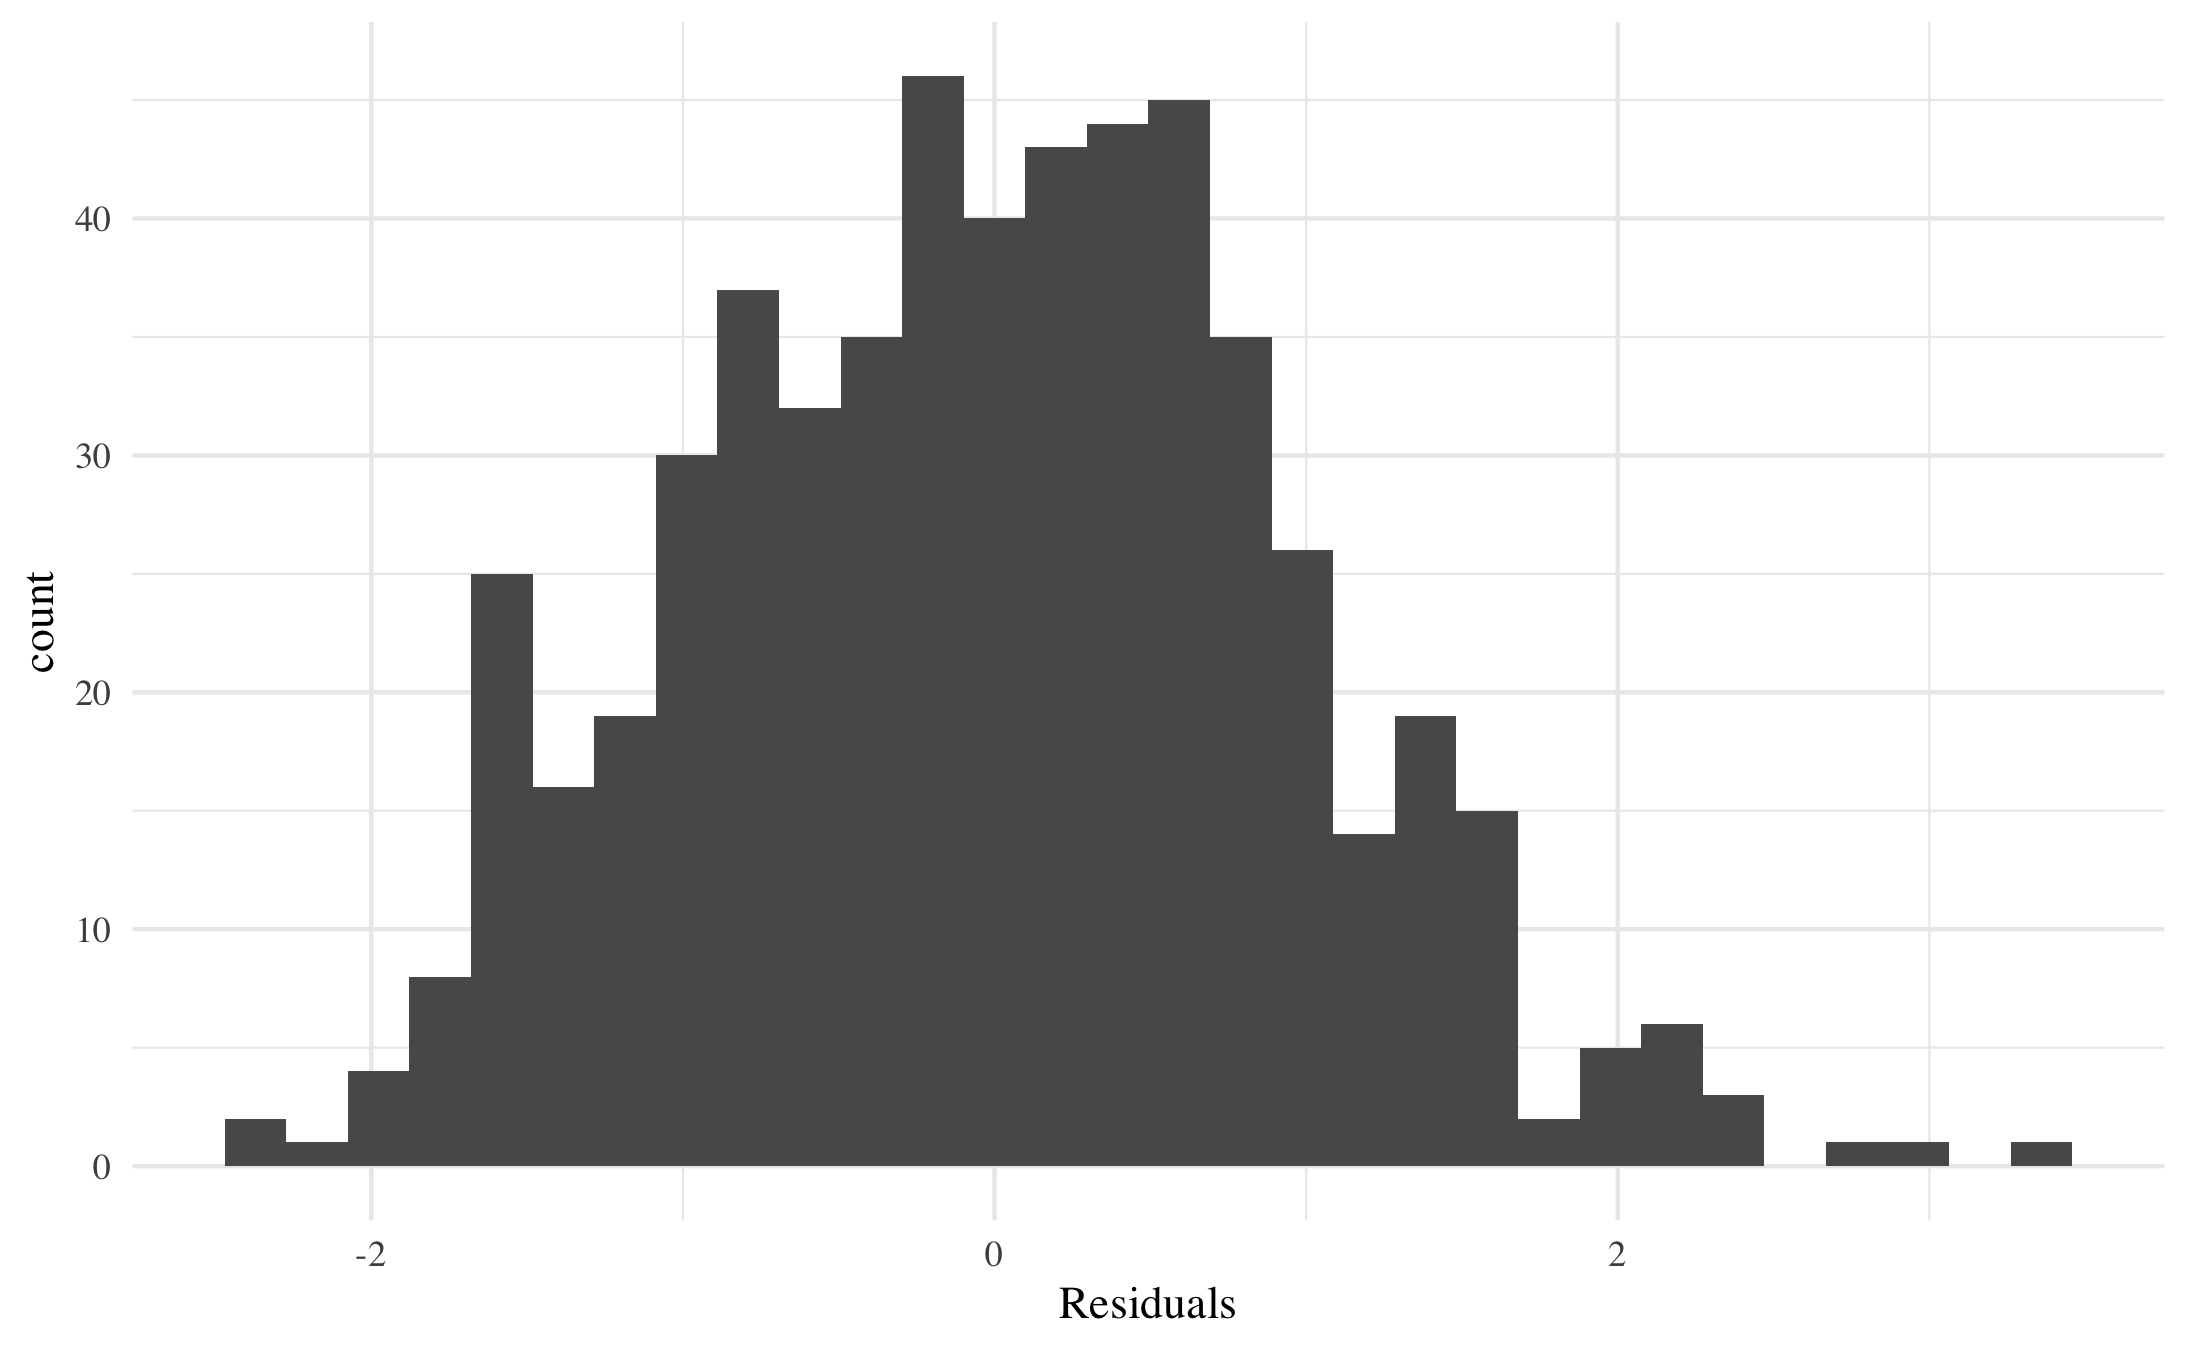
\includegraphics[width=0.9\linewidth]{skew-resids.png}
\caption{Distribution of residuals exhibiting skewness. Pearson's skewness = 0.17. Shapiro-Wilk p-value = 0.08.}
\end{figure}
\end{block}

%----------------------------------------------------------------------------------------

\end{column} % End of column 2.1

\begin{column}{\onecolwid}\vspace{-.6in} % The second column within column 2 (column 2.2)

%----------------------------------------------------------------------------------------
%	METHODS
%----------------------------------------------------------------------------------------

\begin{block}{Full Conditionals}

Let $Y_{i} = \mathbf{x}_i \mathbf{\beta} + \psi z_i + \sigma \epsilon$ with $Z \sim N_+(0,1)$, and $\epsilon \sim N(0,1)$. Define $\mathbf{X}^* = [\mathbf{X} | \mathbf{z}]$, and $\mathbf{\beta}^* = [\beta_0, \beta_1,...,\beta_p, \psi]$. Then,

$$\mathbf{\beta}^*|Y,\mathbf{X}^*,\tau \sim N_{p+2}(\frac{(T_0 \beta_0 + \tau \mathbf{X}^{*T}Y)}{\tau \mathbf{X}^{*T}\mathbf{X}^* + T_0},\tau \mathbf{X}^{*T}\mathbf{X}^* + T_0)$$

$$\tau|\beta^*,\mathbf{X}^{*},Y \sim \Gamma(n/2 + \alpha,\frac{1}{2}(Y-\mathbf{X}^*\beta^*)^T(Y-\mathbf{X}^*\beta^*)+b)$$

$$z_i|y_i,\mathbf{x}_i,\beta,\tau \sim N_+(\frac{\psi \tau(y_i -  \mathbf{x}_i\beta)}{\tau \psi^2 +1},\frac{1}{\tau\psi^2+1})$$

\end{block}

%----------------------------------------------------------------------------------------

\end{column} % End of column 2.2

\end{columns} % End of the split of column 2 - any content after this will now take up 2 columns width

%----------------------------------------------------------------------------------------
%	IMPORTANT RESULT
%----------------------------------------------------------------------------------------

\begin{alertblock}{Important Results}

Through simulation studies, we validated Bayesian Gibbs samplers for skew-normal and skew-t error regression models. We used these models to find an association between birth weight and food security during pregnancy using data from the Nurture study.  

\end{alertblock} 

%----------------------------------------------------------------------------------------

\begin{columns}[t,totalwidth=\twocolwid] % Split up the two columns wide column again

\begin{column}{\onecolwid} % The first column within column 2 (column 2.1)

%----------------------------------------------------------------------------------------
%	MATHEMATICAL SECTION
%----------------------------------------------------------------------------------------

\begin{block}{Modeling Approaches}

\begin{enumerate}
\item \textit{Maximum Likelihood Estimation}: For a random sample $Y_1,Y_2,...,Y_n \stackrel{iid}{\sim} \mathcal{SN}(\xi,\omega^2,\alpha)$, where $\xi = \mathbf{x}^T\beta$ for a collection of predictors $x_1,x_2,...,x_n$ and a vector of unknown regression coefficients $\beta \in {\rm I\!R}^p$. Azzalini (2014) describes procedures for obtaining MLE estimates of $\beta$ and $\alpha$, our primary parameters of interest. Azzalini's {\tt R} package {\tt sn} contains a function {\tt selm} for fitting regression models with $\mathcal{SN}$ or $\mathcal{ST}$ random errors.

\item \textit{Bayesian Gibbs Sampler}: We introduce the following stochastic representation of the skew normal distribution 

$$Y_i = \mathbf{x}_i \beta + \psi z_i + \sigma \epsilon$$

where $z_i \sim N_+(0,1)$ and $\epsilon \sim N(0,1)$. The marginal density of $Y_i$ integrating over $z_i$ and $\epsilon$ is $\mathcal{SN}(\mathbf{x}_i \beta, \omega^2)$. We use this stochastic representation to obtain full conditionals for all parameters. 

\end{enumerate}

\end{block}

%----------------------------------------------------------------------------------------

\end{column} % End of column 2.1

\begin{column}{\onecolwid} % The second column within column 2 (column 2.2)

%----------------------------------------------------------------------------------------
%	RESULTS
%----------------------------------------------------------------------------------------

\begin{block}{Gibbs Sampler Simulation}

\begin{figure}
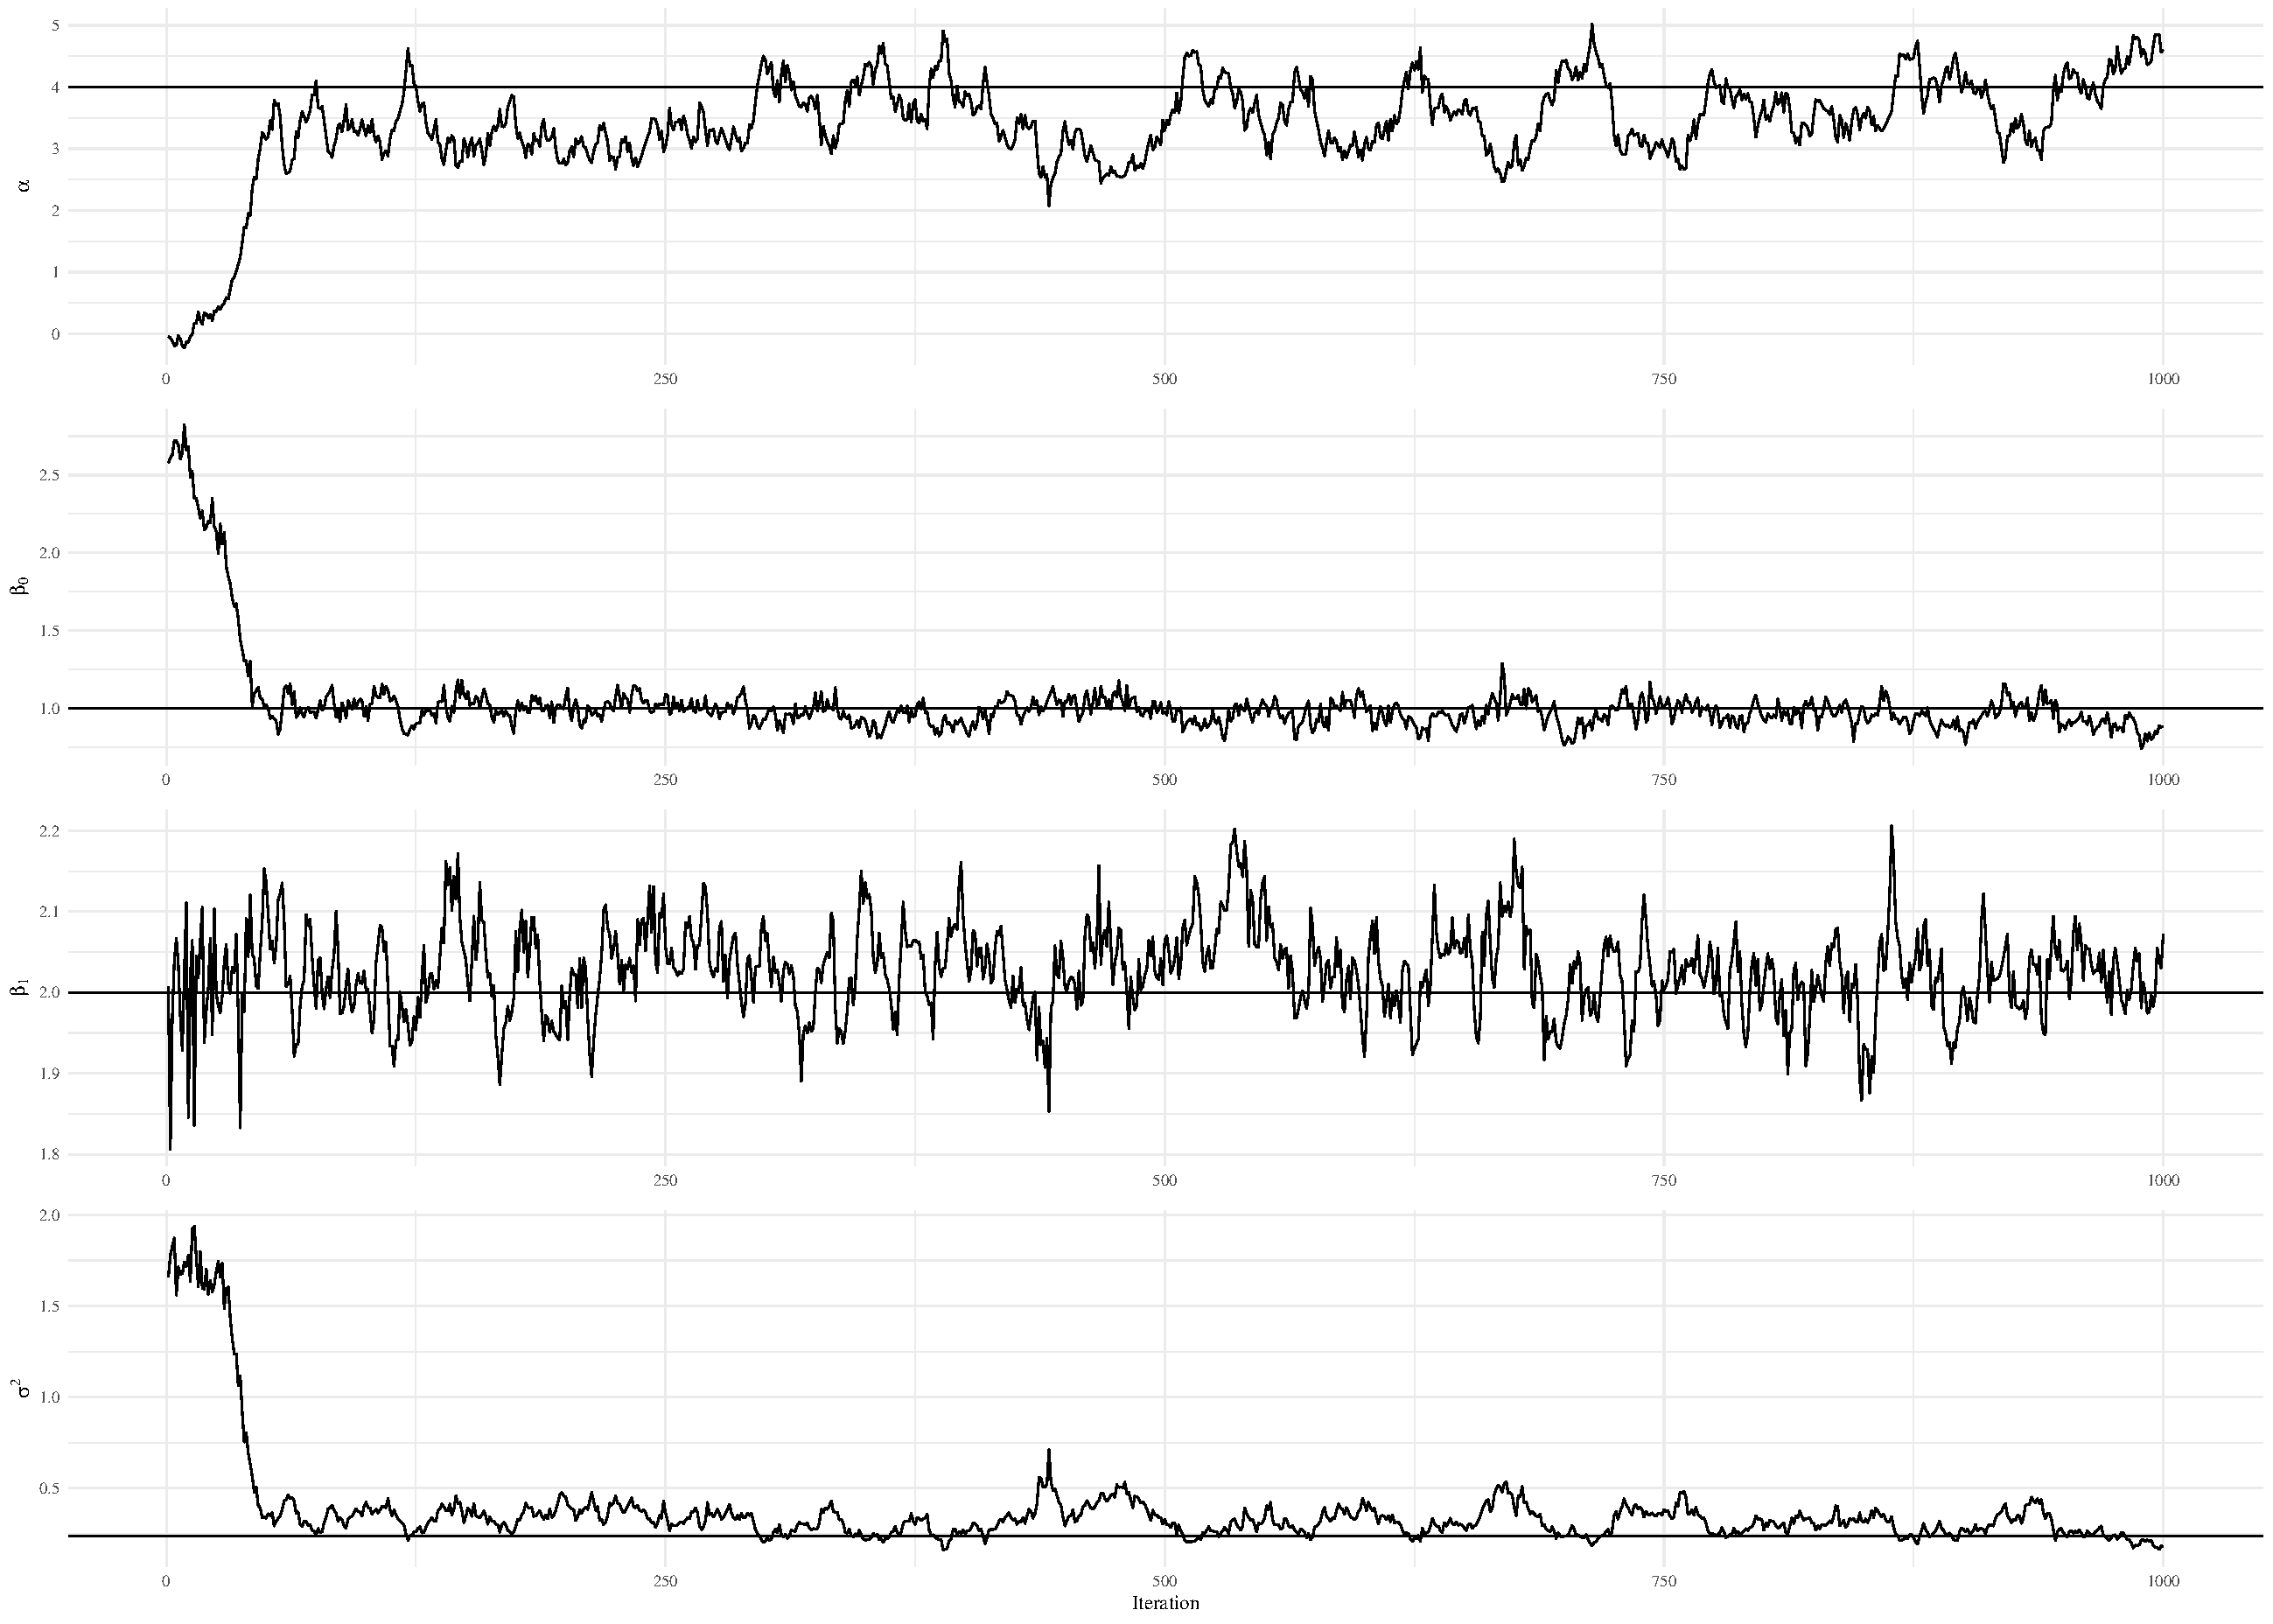
\includegraphics[width=1\linewidth]{sim-trace.pdf}
\caption{Trace plots for skew normal Gibbs sampler simulation}
\end{figure}

\begin{table}
\vspace{0ex}
\begin{tabular}{l l l l}
\toprule
\textbf{Parameter} & \textbf{True} & \textbf{MLE} & \textbf{Gibbs}\\
\midrule
$\alpha$ & 4.00 & 0.3928 & 4.016\\
$\beta_0$ & 1.00 & 1.013 & 1.009\\
$\beta_1$ & 2.00 & 2.006 & 2.01\\
$\sigma^2$ & 0.235 & 0.257 & 0.257\\
\bottomrule
\end{tabular}

\end{table}

\end{block}

%----------------------------------------------------------------------------------------

\end{column} % End of column 2.2

\end{columns} % End of the split of column 2

\end{column} % End of the second column

\begin{column}{\sepwid}\end{column} % Empty spacer column

\begin{column}{\onecolwid} % The third column

%----------------------------------------------------------------------------------------
%	CONCLUSION
%----------------------------------------------------------------------------------------



\begin{figure}
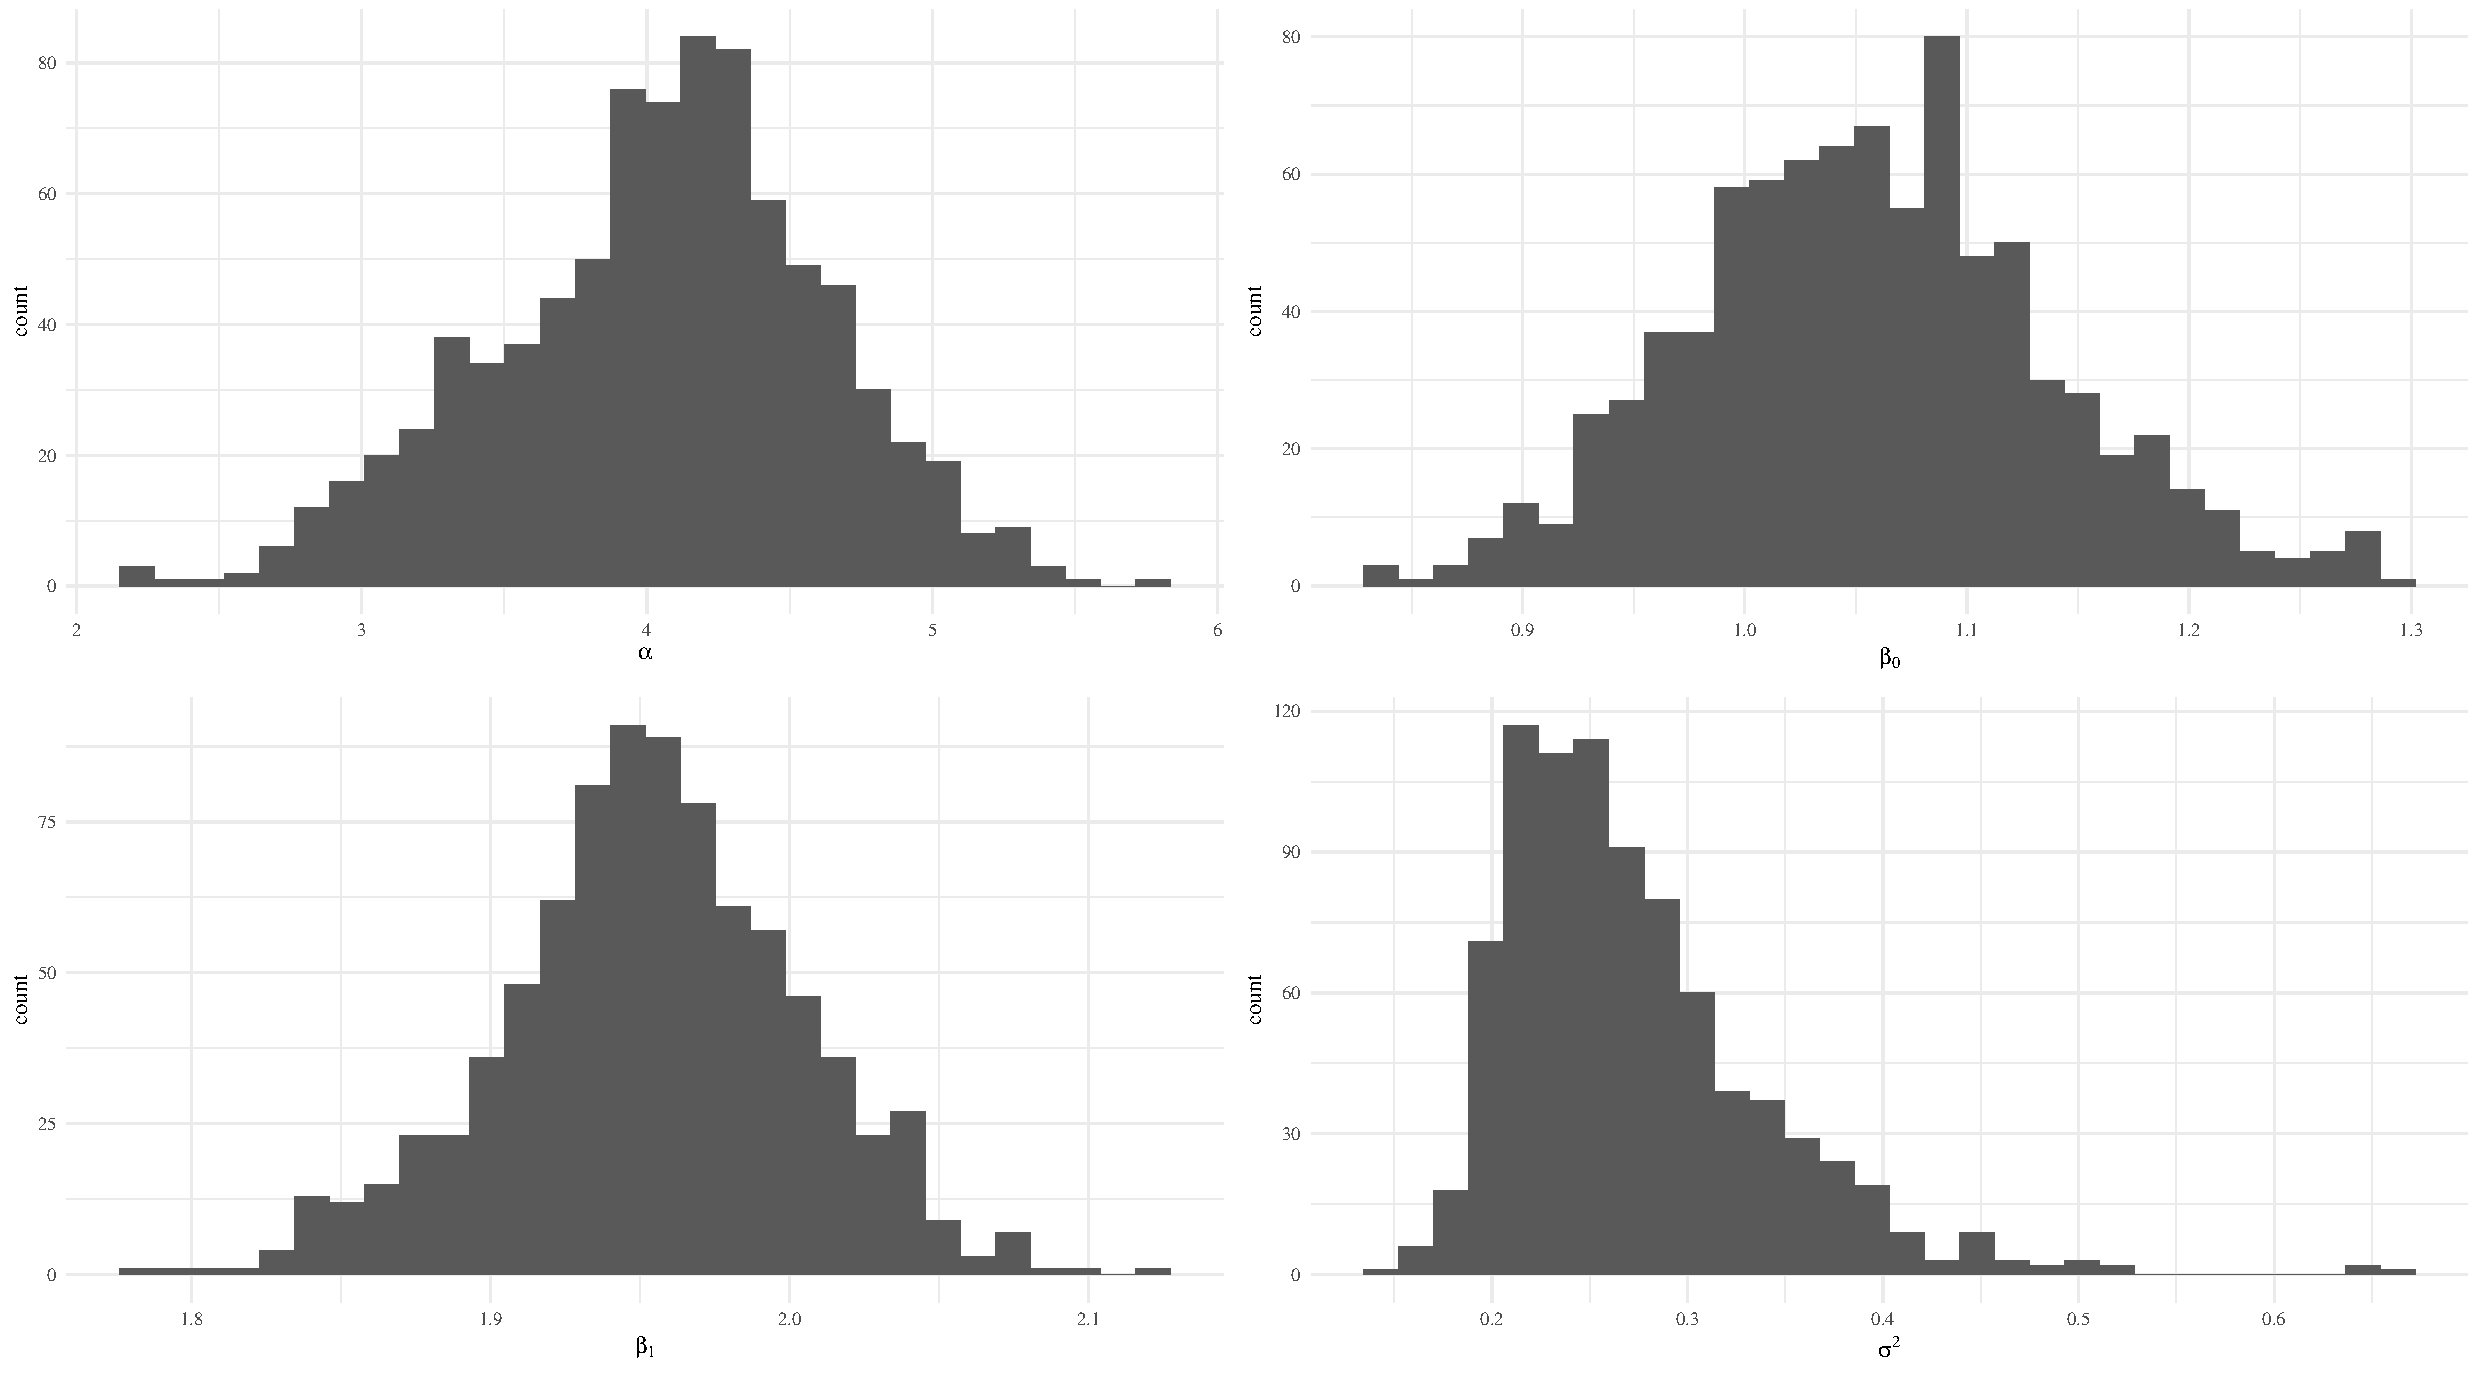
\includegraphics[height=0.8\linewidth,width = 1\linewidth]{sim-post.pdf}
\caption{Simulated posterior distributions}
\end{figure}

\begin{block}{Modeling Results}

\begin{figure}
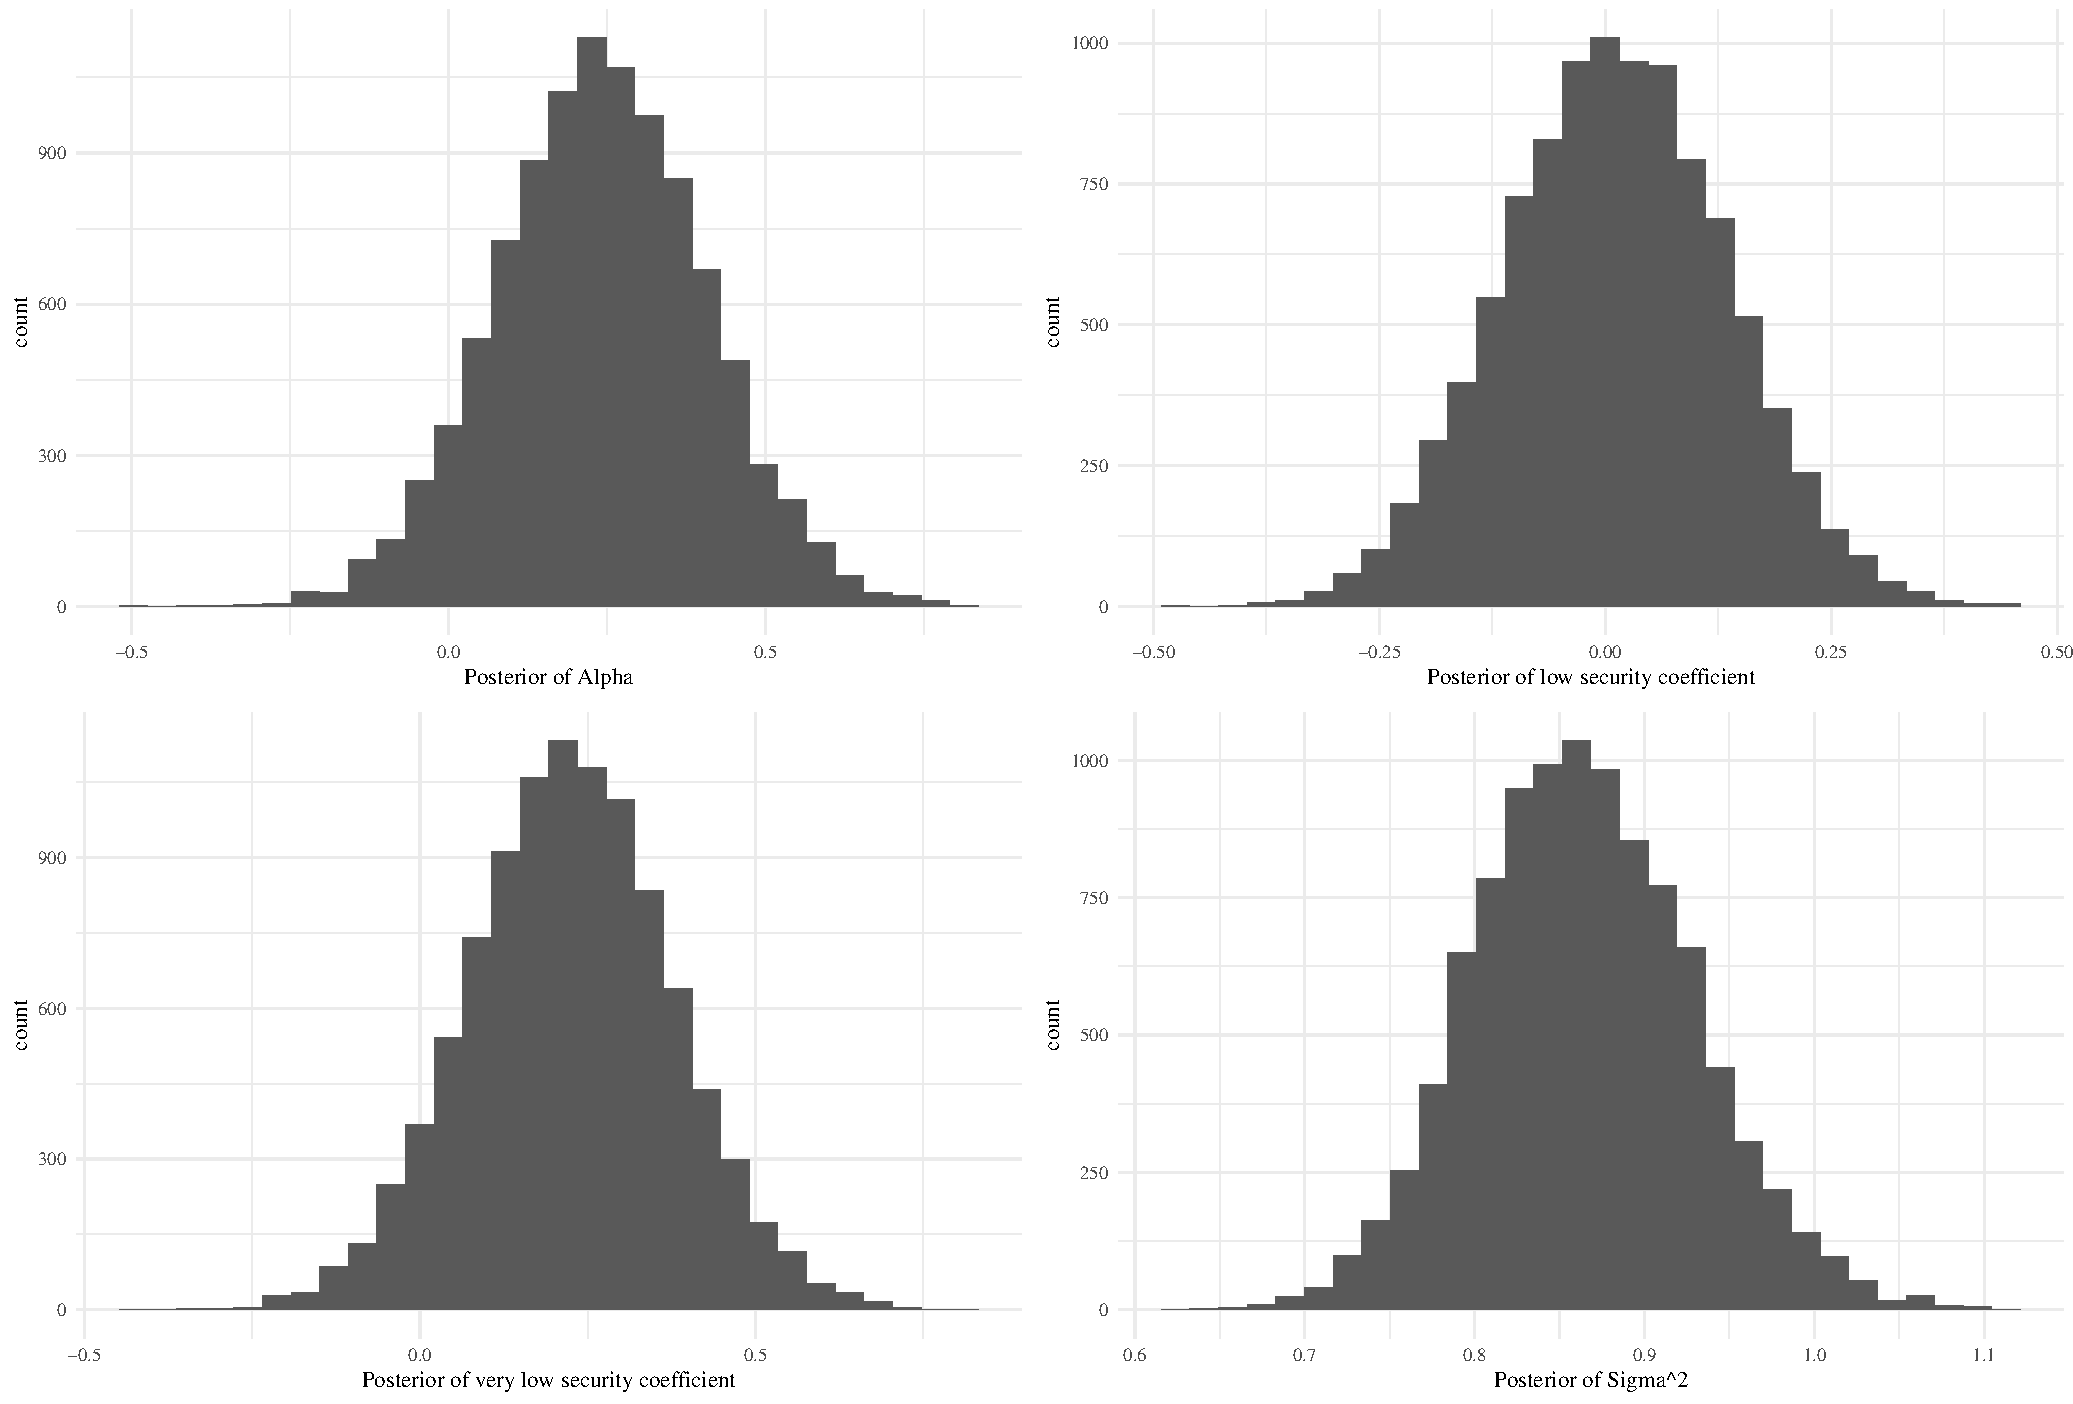
\includegraphics[width=1\linewidth]{nurt_posteriors.pdf}
\caption{Posterior distributions of model parameters}
\end{figure}

\end{block}

\begin{block}{References}

\tiny  \textbf{(1) Azzalini, S. (1985)}. A class of distributions which includes the normal ones. SJS; \textbf{(2) Fruhwirth-Schnatter, S and Pyne, S. (2010)}. Bayesian inference for finite mixtures of univariate ... Biostatistics; \textbf{(3) Benjamin-Neelon SE, Ostbye T, Bennett GG, et al.} Cohort profile for the Nurture Observational Study ... BMJ Open 2017; \textbf{(4) Neelon, B. (2015)} Bayesian two-part spatial models ... Biostatistics.

\end{block}


%----------------------------------------------------------------------------------------
%	REFERENCES
%----------------------------------------------------------------------------------------


%----------------------------------------------------------------------------------------
%	ACKNOWLEDGEMENTS
%----------------------------------------------------------------------------------------


%----------------------------------------------------------------------------------------
%	CONTACT INFORMATION
%----------------------------------------------------------------------------------------

\setbeamercolor{block alerted title}{fg=black,bg=norange} % Change the alert block title colors
\setbeamercolor{block alerted body}{fg=black,bg=white} % Change the alert block body colors

\begin{alertblock}{Further Resources}

\centering
https://carter-allen.github.io/SN

\begin{figure}

\includegraphics[width = .2\linewidth]{frame.png}
\end{figure}

\end{alertblock}

%----------------------------------------------------------------------------------------

\end{column} % End of the third column

\end{columns} % End of all the columns in the poster

\end{frame} % End of the enclosing frame

\end{document}
